\chapter{Specification}

Based on the business requirements we decided that the back-end part of the application must take these five divisions into account: Customers, Employees, Vehicles, Orders and Notifications. In the rest of the chapter we are describing features that these modules should have.
\section{Customers}
Customers are uniquely identified by telephone number. We also want to store about each of them these information:
\begin{itemize}
	\item Name
	\item Image
	\item Note
	\item Fraud status
\end{itemize}
With Customer entity we are able to do these operations:
\begin{itemize}
	\item Create and confirm
	\item Update
	\item Destroy
	\item Recover password
	\item Login and logout
	\item List favorite locations
	\item List all customers and show specific customer
\end{itemize}
\subsection{Operation create}
There are two ways how customer can be created. It is either directly through registration or indirectly by creating new order.

Directly registered customers are created in exchange for telephone number, password and optional name. With this type of account customer can later login with provided password. Application must verify given telephone.

Indirectly registered user is created during creation of new order for telephone number, which doesn't belong to any existing customer. This customer type is just envelop for the purpose of tracking information and statistics - mostly for better customer support. This account type can not be used for authentication. Indirectly registered user can be directly registered later without any difference to normal direct registration.


\subsection{Operation update}
Customer can update only it's own name and password. Employees are able to change any customer's name, note and fraud status.
\subsection{Operation password recovery}
\todo{mention in analysis that we don't want to say whether user exists or not}
In case of lost password is customer able to recover it. At first customer asks for the recovery with its telephone. In return it receives recovery token via SMS. This token is valid for 5 minutes. With this token and telephone number can new password be set. Customer is able to ask for token resend - which will invalidate last token, generate new token and sends it via SMS.
\subsection{Operation login and logout}
With login operation we receive login token in exchange for telephone number and password. We send this token with each request to be authenticated.
Customer can login if and only if is directly registered and confirmed. \todo{in analysis mention that customer can be logged only on one device at time}
\subsection{Operation list favorite locations}

\subsection{Operation list all customers and show specific customer}

\subsection{Employees}
There three types of employees - admins, dispatchers and drivers.
\begin{itemize}
	\item driver locations
	\item shifts
\end{itemize}
\subsection{Vehicles}

\subsection{Orders}

\begin{figure}[h]\centering
	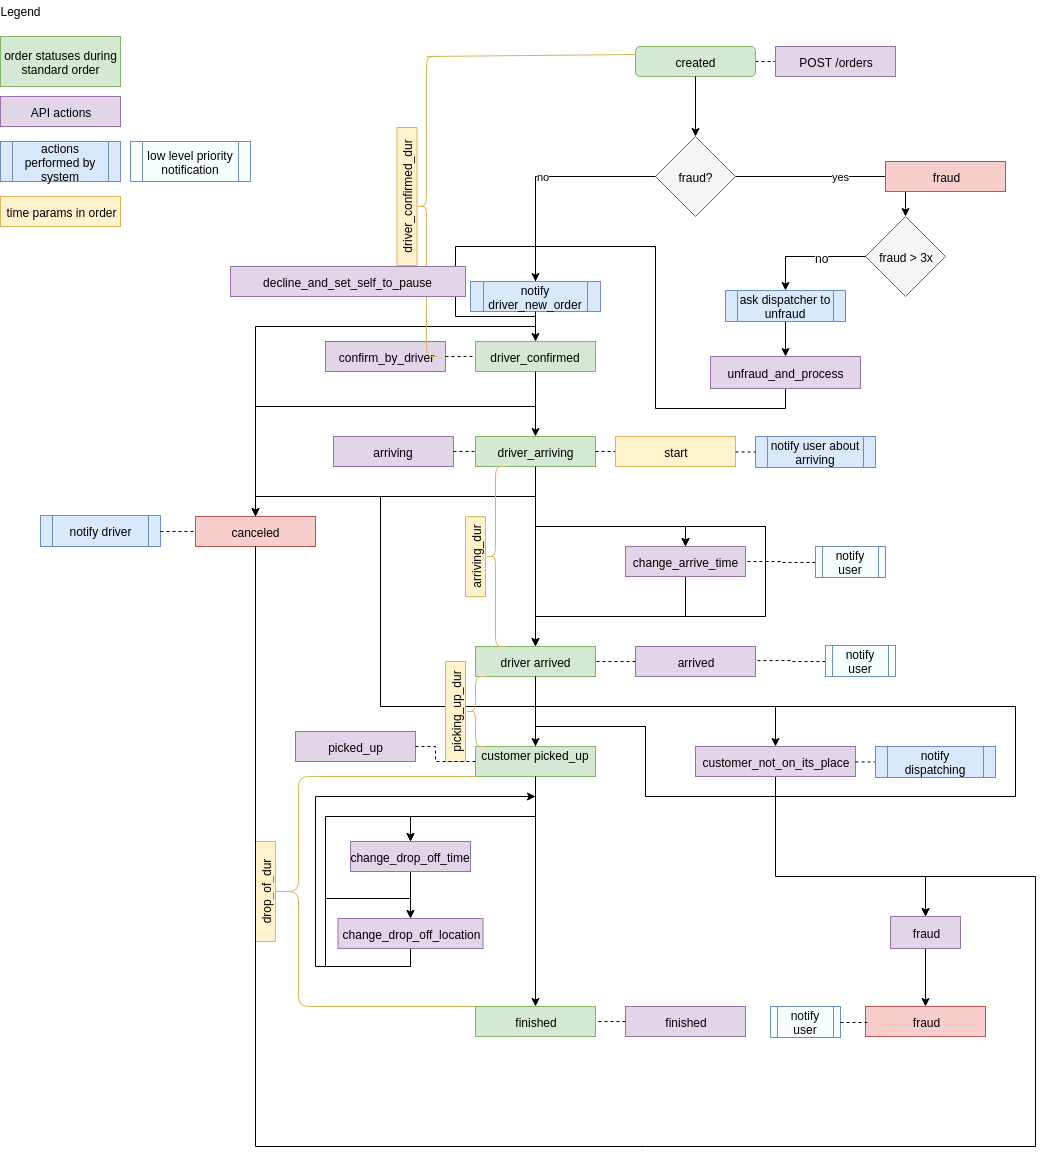
\includegraphics[width=\textwidth]{orders/order_process_scheme.png}
	\caption{Order process scheme}\label{order-process-scheme}
\end{figure}

\begin{figure}[h]\centering
	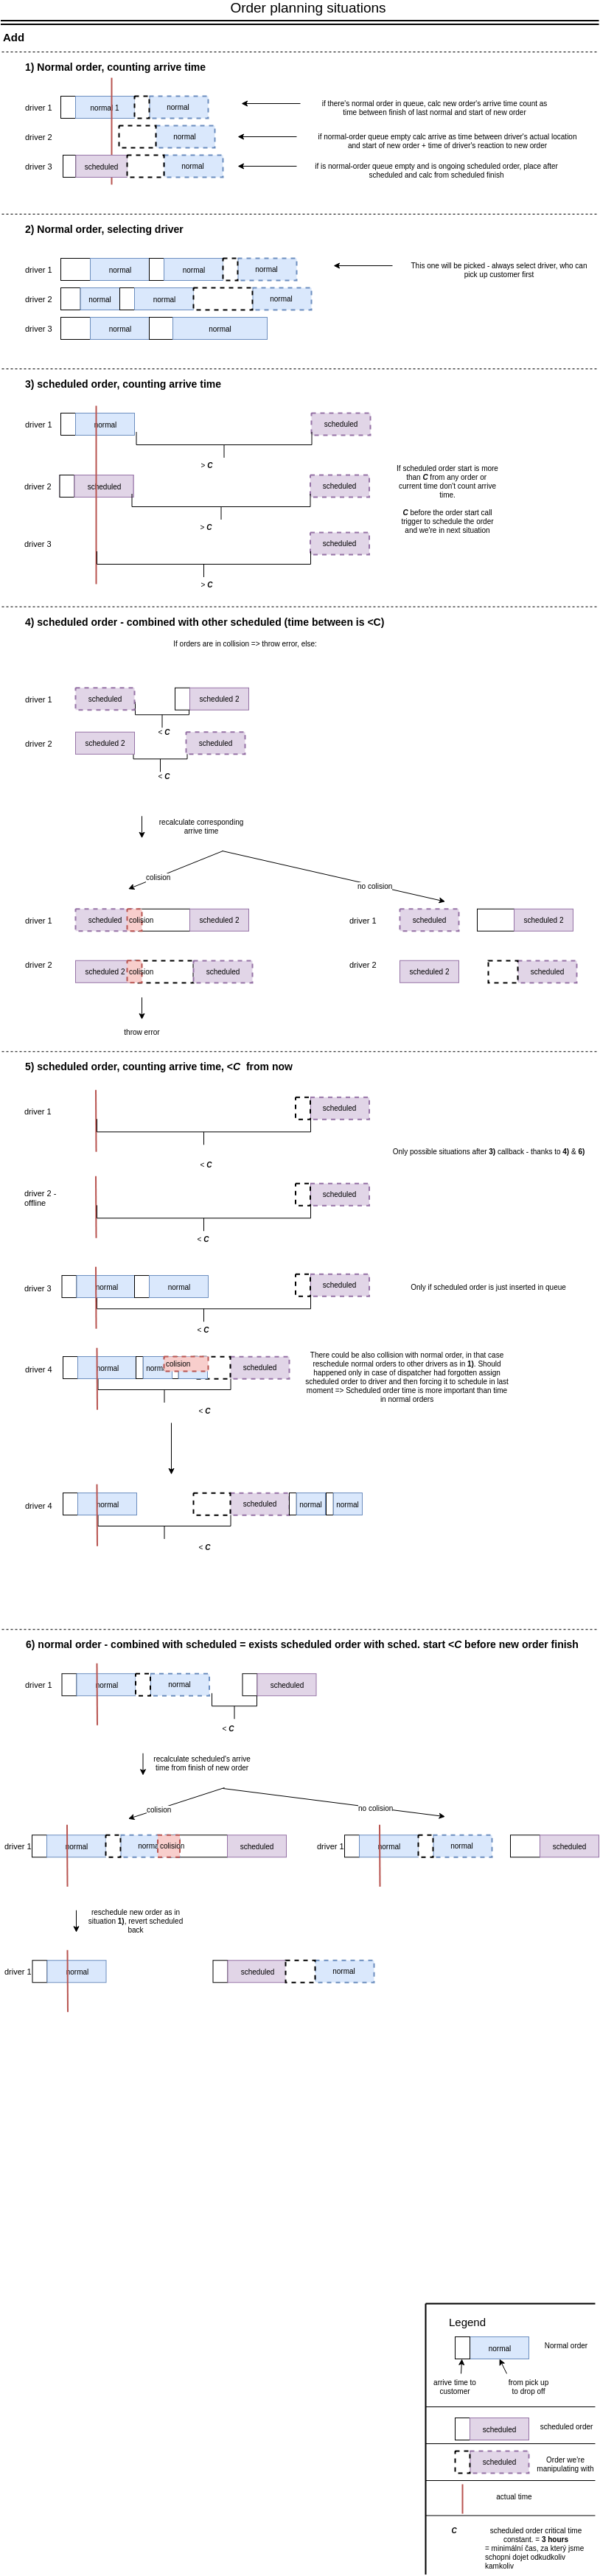
\includegraphics[scale=0.2	]{orders/order_planning.png}
	\caption{Order planning situations}\label{order-process-scheme}
\end{figure} 
\subsection{Notifications}
